\documentclass[10pt]{beamer}

\usetheme{Warsaw}

\usepackage{amsmath}
%\usepackage[style=apa]{biblatex}
\usepackage{multimedia}

\author{George G Vega\thanks{\url{mailto:gvegayon@caltech.edu}}}
\institute{Superintendencia de Pensiones}
\title{An\'alisis de Redes}
\date{20 de junio, 2014}

\begin{document}

\frame{\maketitle}

\begin{frame}
\frametitle{Contenidos}
\tableofcontents
\end{frame}

\section{Introducci\'on}

\begin{frame}
\frametitle{Introducci\'on}
\framesubtitle{Objetivos de esta secci\'on}

Esta parte del curso se centrar\'a en lo siguiente:

\begin{itemize}
\item Familiarizarse con el lenguaje
\item Entender gr\'afos desde mirada estad\'istica
\item Realizar an\'alisis de redes utilizando software especializado (Gephi)
\end{itemize}

\end{frame}

\begin{frame}
\frametitle{Introducci\'on}
\frametitle{Alternativas de software}
\begin{itemize}
\item {\bf UCINET} \url{https://sites.google.com/site/ucinetsoftware/home}
\item {\bf Pajek} \url{http://pajek.imfm.si/doku.php}
\item {\bf NodeXL} \url{http://nodexl.codeplex.com/}
\item {\bf NetworkX} (Python) \url{http://networkx.lanl.gov/}
\item {\bf igraph} (R y otros) \url{http://igraph.org/redirect.html}
\item ...
\item {\bf Gephi} \url{http://gephi.org/}
\end{itemize}
\end{frame}

\begin{frame}
\frametitle{Introducci\'on}
\framesubtitle{La ciencia de redes}

C\'omo se estudian las redes?

\begin{itemize}
\item {\bf Redes biologicas} Redes metab\'olicas, redes regulatorias, etc.
\item {\bf Redes tecnol\'ogicas} Redes de telecomunicaciones, energ\'ia, transporte, etc.
\item {\bf Redes sociales} Amigos, familia, parejas sexuales, etc.
\item {\bf de Informaci\'on} Citas acad\'emicas, World Wide Web (Red), etc.
\end{itemize}

En las ciencias sociales es donde se lleva m\'as tiempo desarrollando
investigaci\'on cuantitativa al respecto.

\end{frame}

\begin{frame}
\frametitle{Introducci\'on}
\framesubtitle{La ciencia de redes}
\begin{figure}
\centering
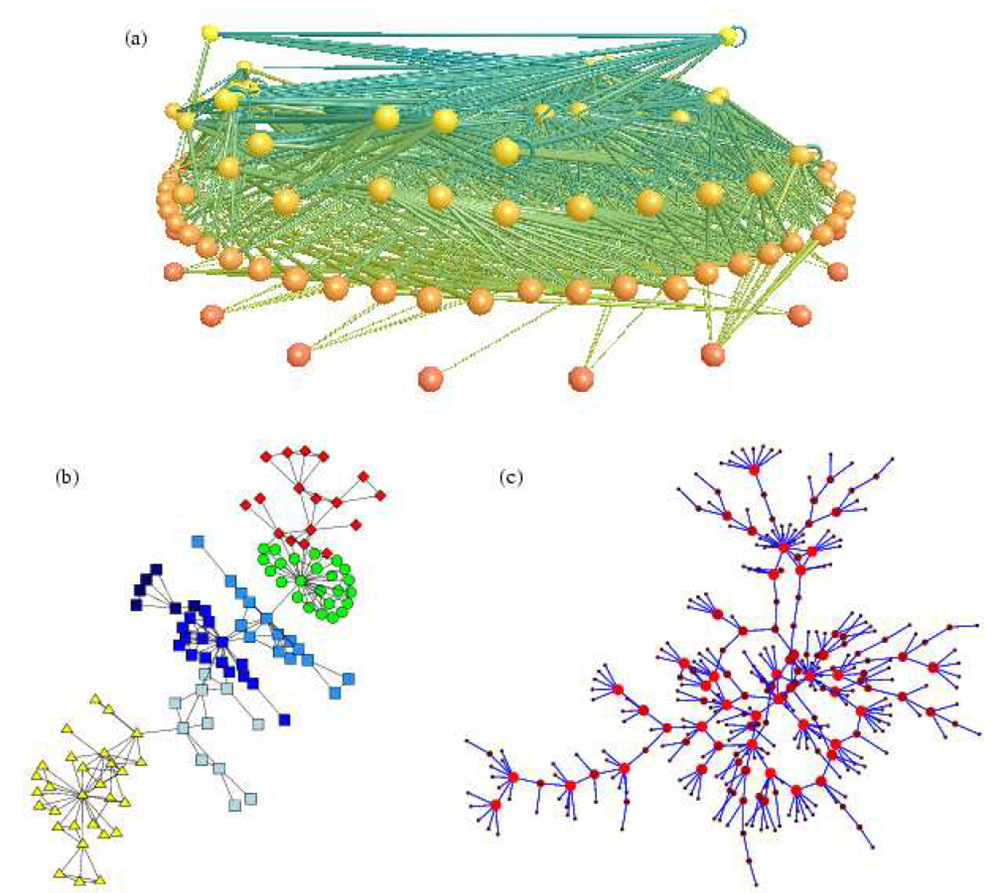
\includegraphics[width =.6\linewidth]{../media/redes_newman_2003.png}
\end{figure}
{\bf a)} Cazador-presa, {\bf b)} Red de colaboraci\'on, y {\bf c)} Red de contactos sexuales
{\footnotesize Fuente: \cite{newman2003structure}}
\end{frame}

\section{Definiciones}

\begin{frame}
\frametitle{Definiciones}

\begin{figure}
\centering
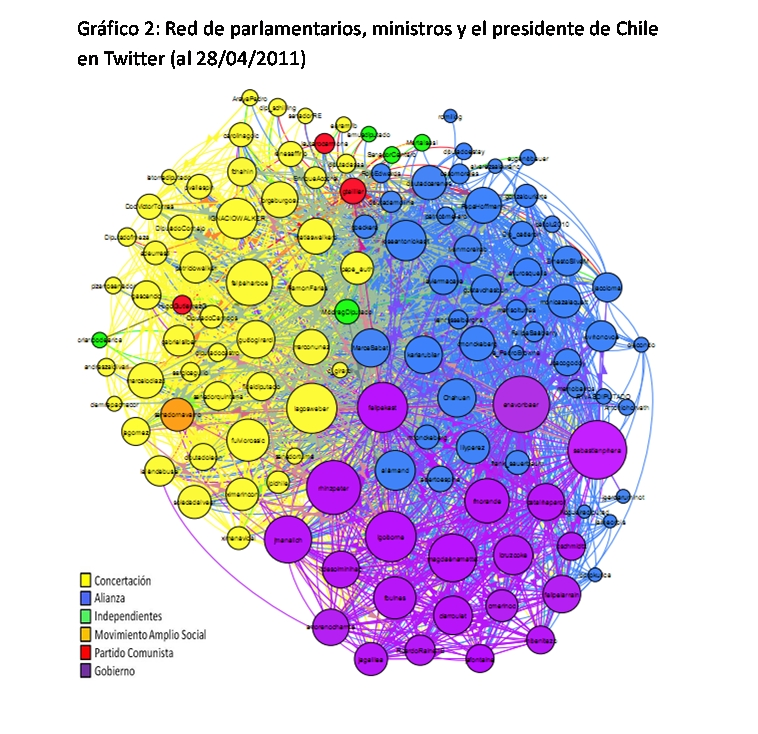
\includegraphics[width=.6\linewidth]{../media/red_parlamentarios_ministros_en_twitter}
\end{figure}
{\footnotesize Fuente: \cite{fabrega2011}}

\end{frame}

\begin{frame}
\frametitle{Definiciones}
\framesubtitle{Conceptos fundamentales}

\begin{itemize}
\item {\bf Vertice} (aka nodo) Unidad fundamental de un grafo.
\item {\bf Arista} (aka arco) Puede ser dirigida o no.
\item {\bf Grado} (entrada/salida) N\'umero de conexiones de un nodo.
\item {\bf Geod\'esica} Distancia m\'as corta entre dos nodos.
\item {\bf Diametro} Distancia m\'as larga en un g\'rafo. 
\item {\bf Diada} Par de nodos conectados.
\item {\bf Triada} Trio de nodos conectados.
\item {\bf Componente} (gigante) Porci\'on de un grafo desconectado.
\end{itemize}
\end{frame}

\begin{frame}
\frametitle{Definiciones}
\framesubtitle{}
\begin{itemize}
\item Definici\'on de gr\'afo: $G = (V,E)$, donde $V$ (vertex) representa el
conjunto de nodos y $E$ (edges) representa el n\'umero de aristas.
\item Tipos de grafo:
  \begin{itemize}
  \item {\bf Grafo vs Bigraf} En un bigrafo existen dos tipos de nodos distintos (personas e instituciones por ejemplo)
  \item {\bf Dirigido} Los arcos tienen sentido, $v_i \rightarrow v_j$
  \item {\bf No dirigido} Los arcos no tienen sentido (direcci\'on), $v_i - v_j$
  \item {\bf C\'iclico} Existen bucles, $v_i \rightarrow v_j \rightarrow v_k \rightarrow v_i$
  \item {\bf a-c\'iclico} No existes bucles
  \end{itemize}
\end{itemize}

\end{frame}

\begin{frame}
\frametitle{Definiciones}
\framesubtitle{Caracterizando una red}

M\'aximo n\'umero de conexiones en un grafo {\bf dirigido}
\begin{equation}
n(n-1)
\end{equation}

M\'aximo n\'umero de conexiones en un grafo {\bf no dirigido}
\begin{equation}
\frac{1}{2}n(n-1)
\end{equation}
\end{frame}

\begin{frame}
\frametitle{Definiciones}
\framesubtitle{Mundos Peque\~nos}

{\bf efecto mundo-peque\~no} el hecho de que la mayor\'ia de los pares de
nodos est\'a conectado por un camino peque\~no a lo largo del grafo.

La primera evidencia de esto se encuentra en el experimento de Stanley Milgram
\cite{milgram1967} 

Se puede medir en funci\'on de la geod\'esica media

\begin{equation}
\ell = \frac{1}{\frac{1}{2}n(n+1)}\sum_{i\geq j}{d_{ij}}
\end{equation}

Notar que $\frac{1}{2}n(n+1)$ corresponde al m\'aximo n\'umero de links
posibles.

Como $d_{ij} \rightarrow \infty$, se recomienda calcular

\begin{equation}
\ell^{-1} = \frac{1}{\frac{1}{2}n(n+1)}\sum_{i\geq j}{d_{ij}^{-1}}
\end{equation}

\end{frame}

\begin{frame}
\frametitle{Definiciones}
\framesubtitle{Distribuci\'on de grado}
Una caracter\'istica importante de los grafos \emph{naturales} es la distribuci\'on
del grado ($k_i$) de sus nodos ($v_i$)

\begin{equation*}
\text{P(grado$\geq k$)} : P_k = \sum_{k' = k}^{\infty}{p_k'}
\end{equation*}
\noindent donde $p_k$ es la fracci\'on de nodos que tiene grado $k$

\noindent Ahora, dado que se da $p_k \sim k^{-\alpha}$

\begin{equation*}
P_k \sim \sum_{k'=k}^{\infty}{k^{-\alpha}} \sim k^{-(\alpha - 1)}
\end{equation*}

\end{frame}

\begin{frame}
\frametitle{Definiciones}
\framesubtitle{Distribuci\'on de grado}
\begin{figure}
\centering
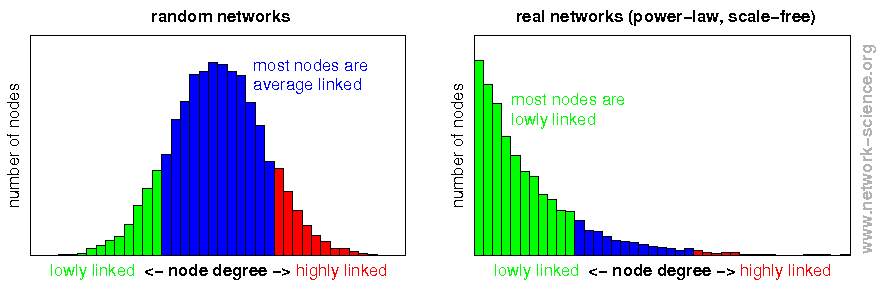
\includegraphics[width=\linewidth]{../media/node_degree_distribution.png}
\end{figure}
\end{frame}

\section{Estad\'isticos}

\begin{frame}
\frametitle{Definiciones}
\framesubtitle{Clusterizaci\'on}

Indica en qu\'e medida existen triadas conectadas en un grafo.

\begin{itemize}
\item {\bf Watts y Strogratz, 1998}
\begin{equation}
C_i = \frac{2E_i}{k_i(k_i - 1)} ; C = \frac{1}{n}\sum_{i \in V}{C_i}
\end{equation}
\noindent donde $E_i$ corresponde al n\'umero de arcos, $k_i$ el grado del nodo
$i$.
\item {\bf Barrat y Weight, 2000; Newman, Strogatz y Watts, 2000}
\begin{equation}
C = \frac{3 \times \text{\# de triangulos en el grafo}}{\text{\# de triadas}}
\end{equation}
\end{itemize}

El n\'umero 3 se utiliza para asegurar que el \'indice se encuentre entre 0 y 1

\end{frame}

\begin{frame}
\frametitle{Definiciones}
\framesubtitle{Clusterizaci\'on}
\begin{figure}
\centering
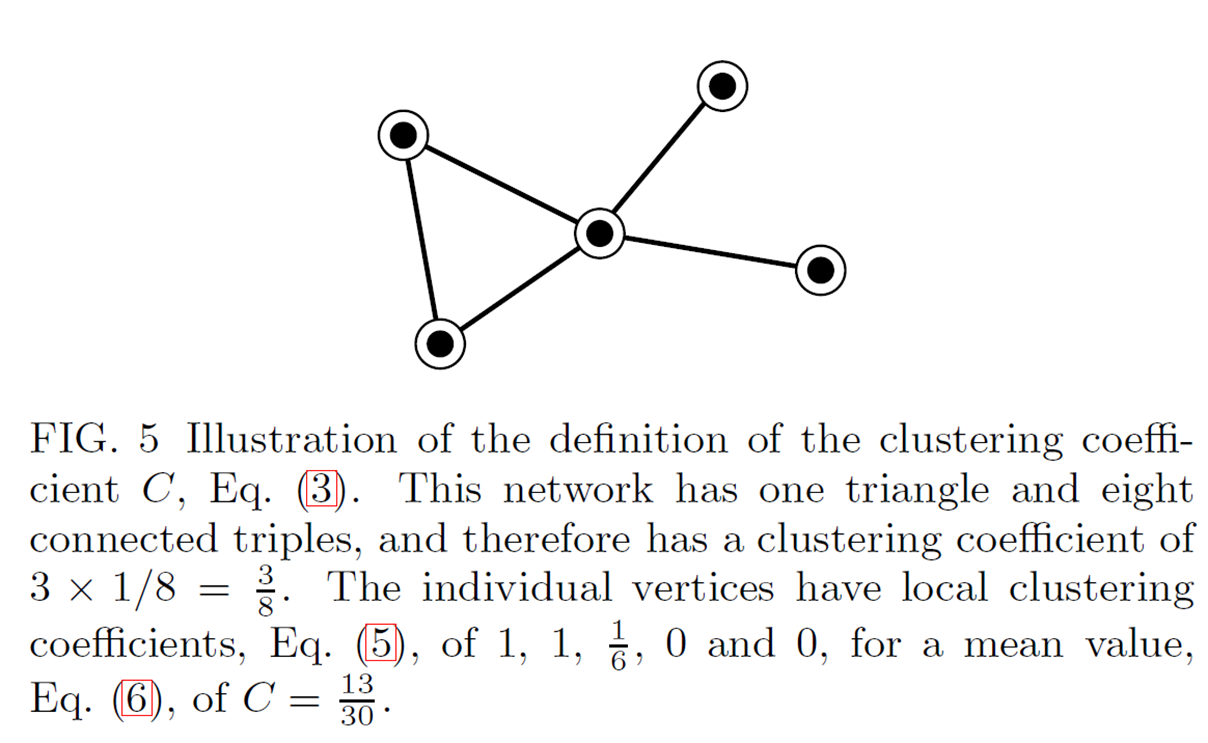
\includegraphics[width=.6\linewidth]{small_net_centrality.png}
\end{figure}

{\bf (3.3)} Nuestra ecuaci\'on (6); {\bf (3.5)} y  {\bf (3.6)} Nuestra ecuaci\'on (5)

\end{frame}

\section{Ejemplos}

\begin{frame}
\frametitle{Ejemplos}
\framesubtitle{Medidas en la literatura}
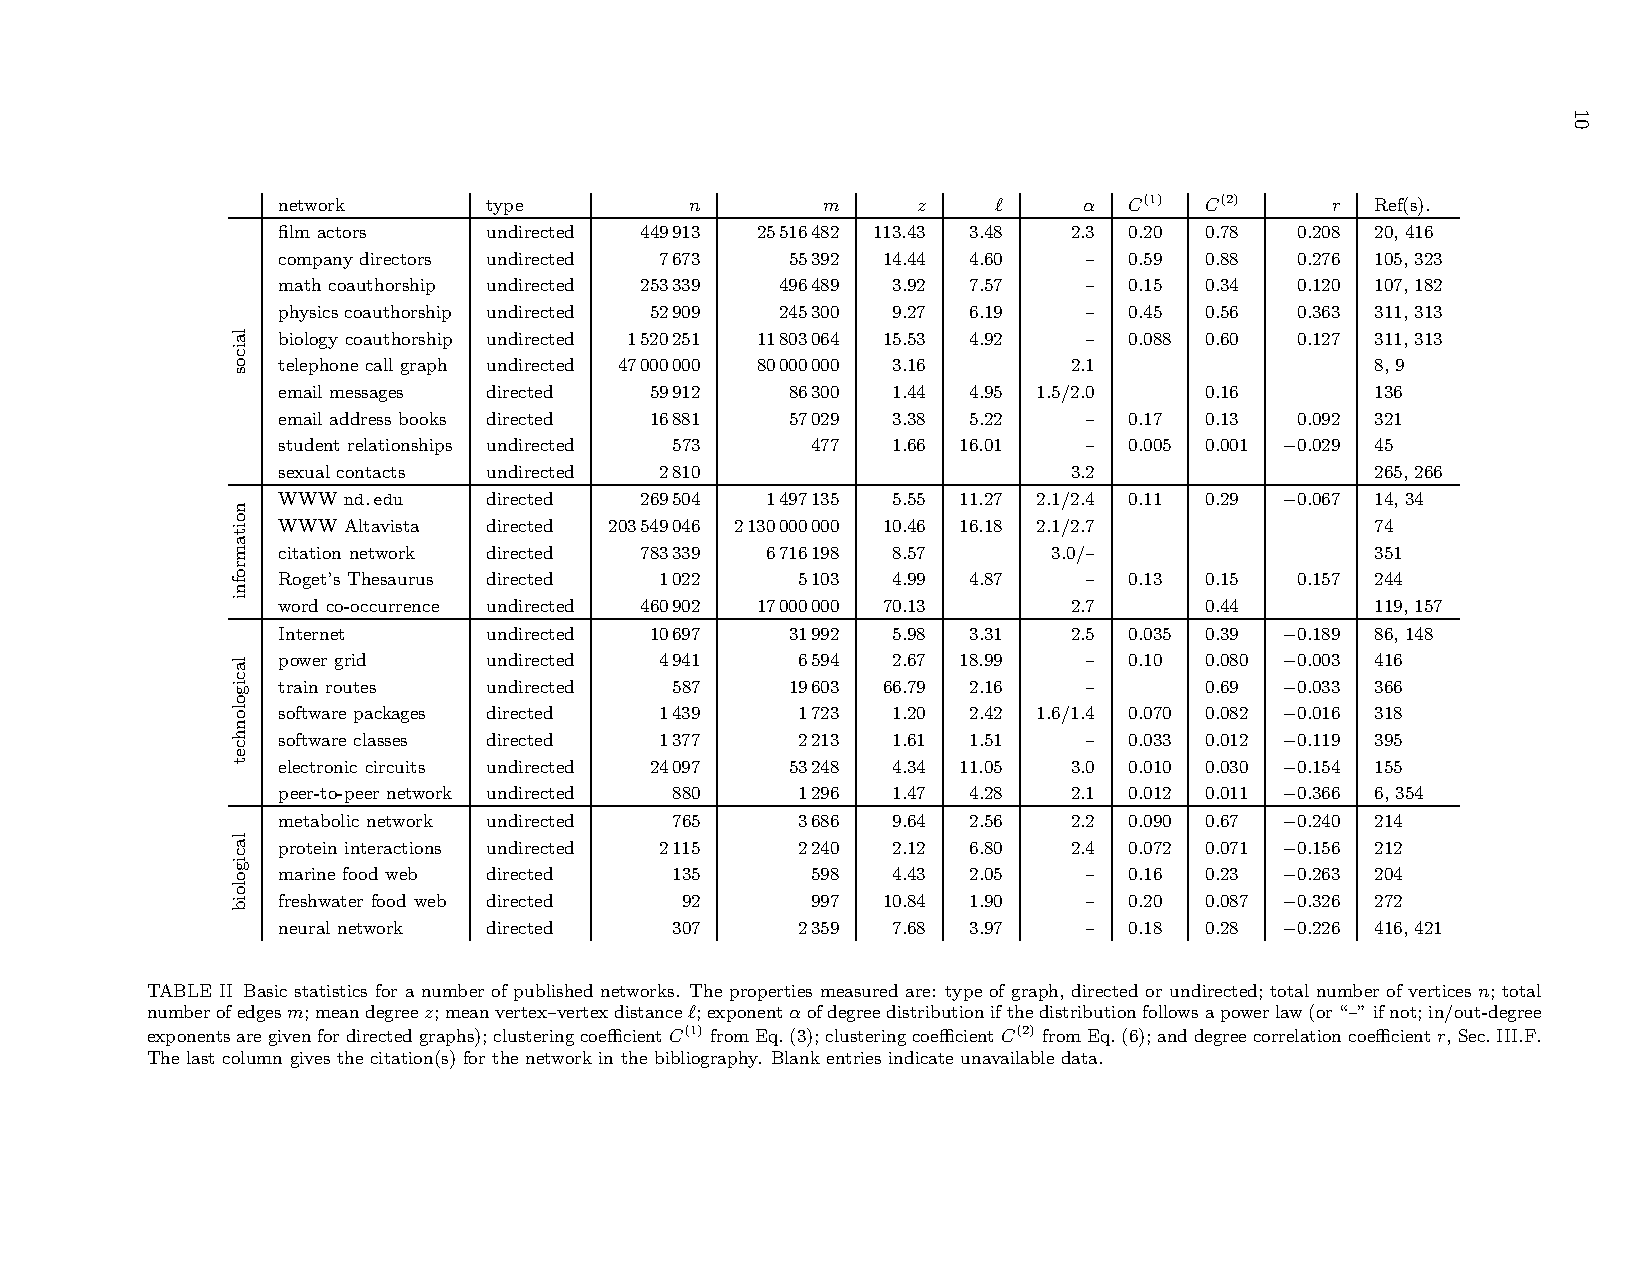
\includegraphics[trim=1cm 1.5cm 1cm 1.5cm, clip=true, width=\linewidth]{the_structure_and_function_of_complex_networks_(newman_2003)_tabla_ii.pdf}
%\movie[options]{placeholder box}{movie filename}
\end{frame}

\begin{frame}
\frametitle{Temas que revisaremos en la pr\'oxima sesi\'on}
\begin{itemize}
\item Centralidad de Grado (in/out)
\item Centralidad de Cercan\'ia
\item Centralidad de Intermediaci\'on
\end{itemize}
Otras medidas de centralidad...
\begin{itemize}
\item N\'umero de Erd{\"o}s 
\item El or\'aculo de Kevin Bacon \url{http://oracleofbacon.org/}
\end{itemize}
\end{frame}

\section{Referencias}
\begin{frame}
\frametitle{Referencias}
\bibliographystyle{plain}
\bibliography{../bib}
\end{frame}


\end{document}

